\documentclass[xcolor=x11names,compress]{beamer}

% Packages
\usepackage{graphicx}
\usepackage{tikz}
\usetikzlibrary{decorations.fractals}
\usepackage{hyperref}
\usepackage{mathrsfs}
\usepackage[mathcal]{euscript}
\usepackage{amssymb}
\usepackage{amsthm}
\usepackage{epsfig}
\usepackage{amsmath}
\usepackage{wrapfig}
\usetikzlibrary{arrows,decorations.pathmorphing}
\usepackage{media9}
%\usepackage[font=footnotesize,labelfont=bf,labelsep=period]{caption}

%remove the icon
\setbeamertemplate{bibliography item}{}

%remove line breaks
\setbeamertemplate{bibliography entry title}{}
\setbeamertemplate{bibliography entry location}{}
\setbeamertemplate{bibliography entry note}{}

% Beamer Layout
\useoutertheme[subsection=false,shadow]{miniframes}
\useinnertheme{default}
\usefonttheme{serif}
\usepackage{palatino}
\usepackage{tabu}
\setbeamerfont{title like}{shape=\scshape}
\setbeamerfont{frametitle}{shape=\scshape}
\setbeamertemplate{frametitle}{\color{black}\bfseries\insertframetitle\par\vskip-6pt\hrulefill}
\setbeamerfont{caption}{size=\tiny}

% Links
\usepackage{hyperref}
\definecolor{links}{HTML}{003262}
\hypersetup{colorlinks,linkcolor=,urlcolor=links}

% Colors
\usepackage{color}
\usepackage{xcolor}
\definecolor{lightblue}{RGB}{65,120,225}
\definecolor{mediumblue}{RGB}{0,0,205}
\definecolor{darkblue}{RGB}{0,0,120}
\definecolor{berkeleyblue}{HTML}{003262}
\definecolor{berkeleygold}{HTML}{FDB515}
\setbeamercolor*{lower separation line head}{bg=black}
\setbeamercolor*{normal text}{fg=black,bg=white}
\setbeamercolor*{alerted text}{fg=black}
\setbeamercolor*{example text}{fg=black}
\setbeamercolor*{structure}{fg=black}
\setbeamercolor*{palette tertiary}{fg=black,bg=black!10}
\setbeamercolor*{palette quaternary}{fg=black,bg=black!10}

% Margins
\usepackage{changepage}


\mode<presentation>
{
  \usetheme{Boadilla}      % or try Darmstadt, Madrid, Warsaw, Boadilla
  %\usecolortheme{dove} % or try albatross, beaver, crane
  \setbeamercolor{structure}{fg=black,bg=white}
  \setbeamercolor{palette primary}{bg=mediumblue, fg=white}
  \setbeamercolor{palette secondary}{bg=lightblue, fg=white}
  \setbeamercolor{palette tertiary}{bg=darkblue, fg=white}
  \usefonttheme{serif}
  \useinnertheme{circles}
  \setbeamertemplate{navigation symbols}{}
  \setbeamertemplate{caption}[numbered]

  \usebackgroundtemplate{}
}

\renewcommand{\(}{\begin{columns}}
\renewcommand{\)}{\end{columns}}
\newcommand{\<}[1]{\begin{column}{#1}}
\renewcommand{\>}{\end{column}}


%% Adding slide numbers
%\addtobeamertemplate{navigation symbols}{}{%
%    \usebeamerfont{footline}%
%    \usebeamercolor[fg]{footline}%
%    \hspace{1em}%
%    \insertframenumber/\inserttotalframenumber
%}


%------------------------------------------------------------------------------------------------------
% Title and authors
\title[NE 255 - Final Project]{Monte Carlo Simulation and Reconstruction Framework for a CdZnTe-based Spherical Coded Aperture and Compton Gamma-ray Imager}
%\subtitle{Subtitle}
\author{D. Hellfeld}
\institute[UC Berkeley]{NE 255 - Numerical Simulation in Radiation Transport \\ University of California, Berkeley \\ Department of Nuclear Engineering}
\date{December 14, 2016}


\begin{document}

%------------------------------------------------------------------------------------------------------
\begin{frame}
\maketitle
\end{frame}


%------------------------------------------------------------------------------------------------------
\begin{frame}{Outline}
\begin{itemize} \setlength\itemsep{1.3em}
\item Introduction
\item Coded Aperture Imaging
\item Compton Imaging
\item Monte Carlo Simulation - Geant4
\item Results
\item Conclusions/Future Work
\end{itemize}
\end{frame}



%------------------------------------------------------------------------------------------------------
\begin{frame}{Introduction}

\textcolor{blue}{\textbf{Motivation}}\\
Efficiently detect, image, identify, and characterize weak radioactive sources in complex environments.
\begin{itemize}
\small
\item[-] Applications in astronomy, medical imaging, and \textbf{nuclear security}.
%(treat verification, safeguards, source search, contamination remediation).
\end{itemize}

\vspace{15pt}
\textcolor{blue}{\textbf{Need}}\\
Hand-held, portable 3D imaging system with high efficiency, wide field-of-view, broad energy sensitivity, and high energy resolution.\\

\vspace{15pt}
\textcolor{blue}{\textbf{Approach}}\\
Multiple room-temperature operated cm$^3$ CdZnTe (CZT) coplanar gird (CPG) \cite{Luke} detectors arranged to facilitate coded aperture and Compton imaging modalities.  


\end{frame}


%------------------------------------------------------------------------------------------------------
\begin{frame}{Coded Aperture Imaging - Concept}

\begin{figure}
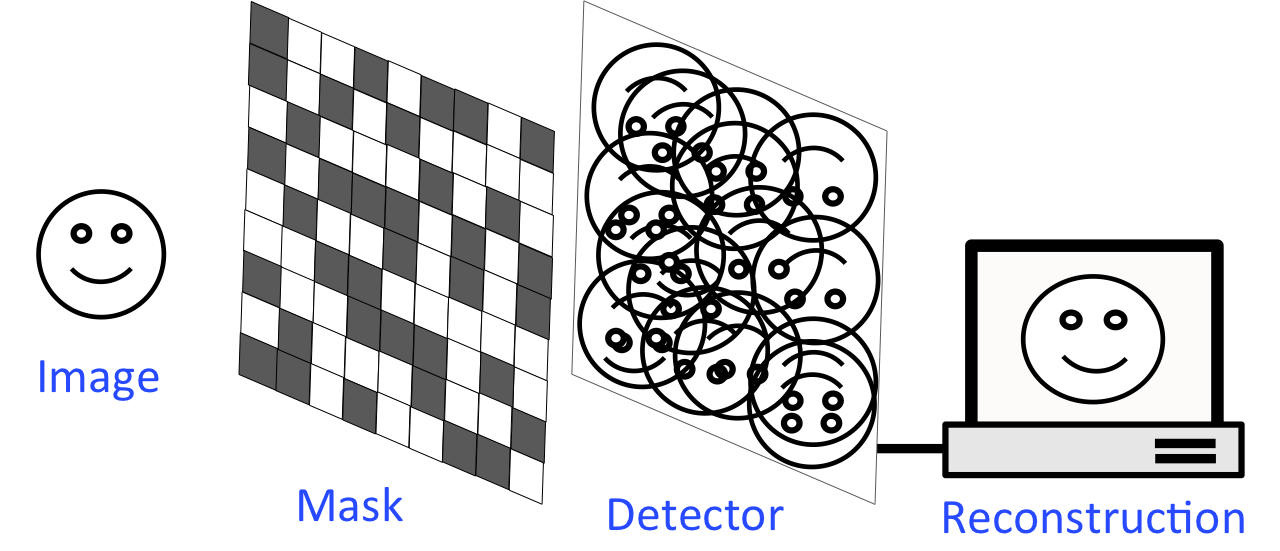
\includegraphics[height=2in]{Figures/Smiley.png}
\end{figure}

The mask modulates photon flux to create detectable \emph{shadowgrams} that are unique to each point in the image space.

\end{frame}



%------------------------------------------------------------------------------------------------------
\begin{frame}{Coded Aperture Imaging - Image Recon.}


Fast analytical reconstruction methods exist (simple back-projection, filtered back-projection, cross-correlation) \cite{Wahl,Fenimore}
\begin{itemize}
\item[$\circ$] Most fail to include relevant physics, produce blurry images.
\end{itemize}

\vspace{1ex}
Focus on iterative method - \textbf{Maximum Likelihood Expectation Maximization (MLEM)} \cite{Lange}


\vspace{-15pt}
 \begin{align*}
	\lambda_j^{n+1} = \frac{\lambda_j^n}{\sum\limits_{i \in J_j}C_{ij}} \sum_{i \in J_j} \frac{C_{ij}g_i}{\sum\limits_{k \in I_i}C_{ik}\lambda_k^n}\
\end{align*}

\vspace{-10pt}

\begin{itemize}
\small
\item[-] $C_{ij}$ is the probability an event in detector $i$ came from image pixel $j$
\item[-] $g_i$ are the counts in detector $i$
\item[-] $\lambda_j^n$ is the intensity of image pixel $j$ for iteration $n$
\item[-] $I_i$ are the set of image pixels that contribute to detector $i$
\item[-] $J_j$ are the set of detectors to which image pixel $j$ contributes
\end{itemize}
\end{frame}



%------------------------------------------------------------------------------------------------------
\begin{frame}{Compton Imaging - Concept}

\vspace{-10pt}

\begin{figure}
\begin{tabular}{ccc}
&& \cite{Haefner} \\[-3ex]
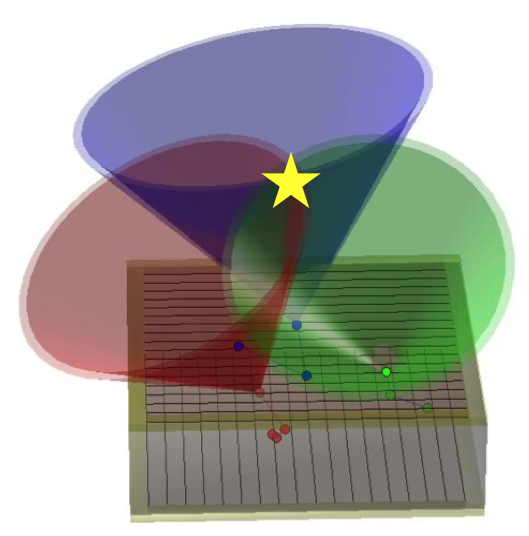
\includegraphics[height=1.7in]{Figures/Compton.png} & 
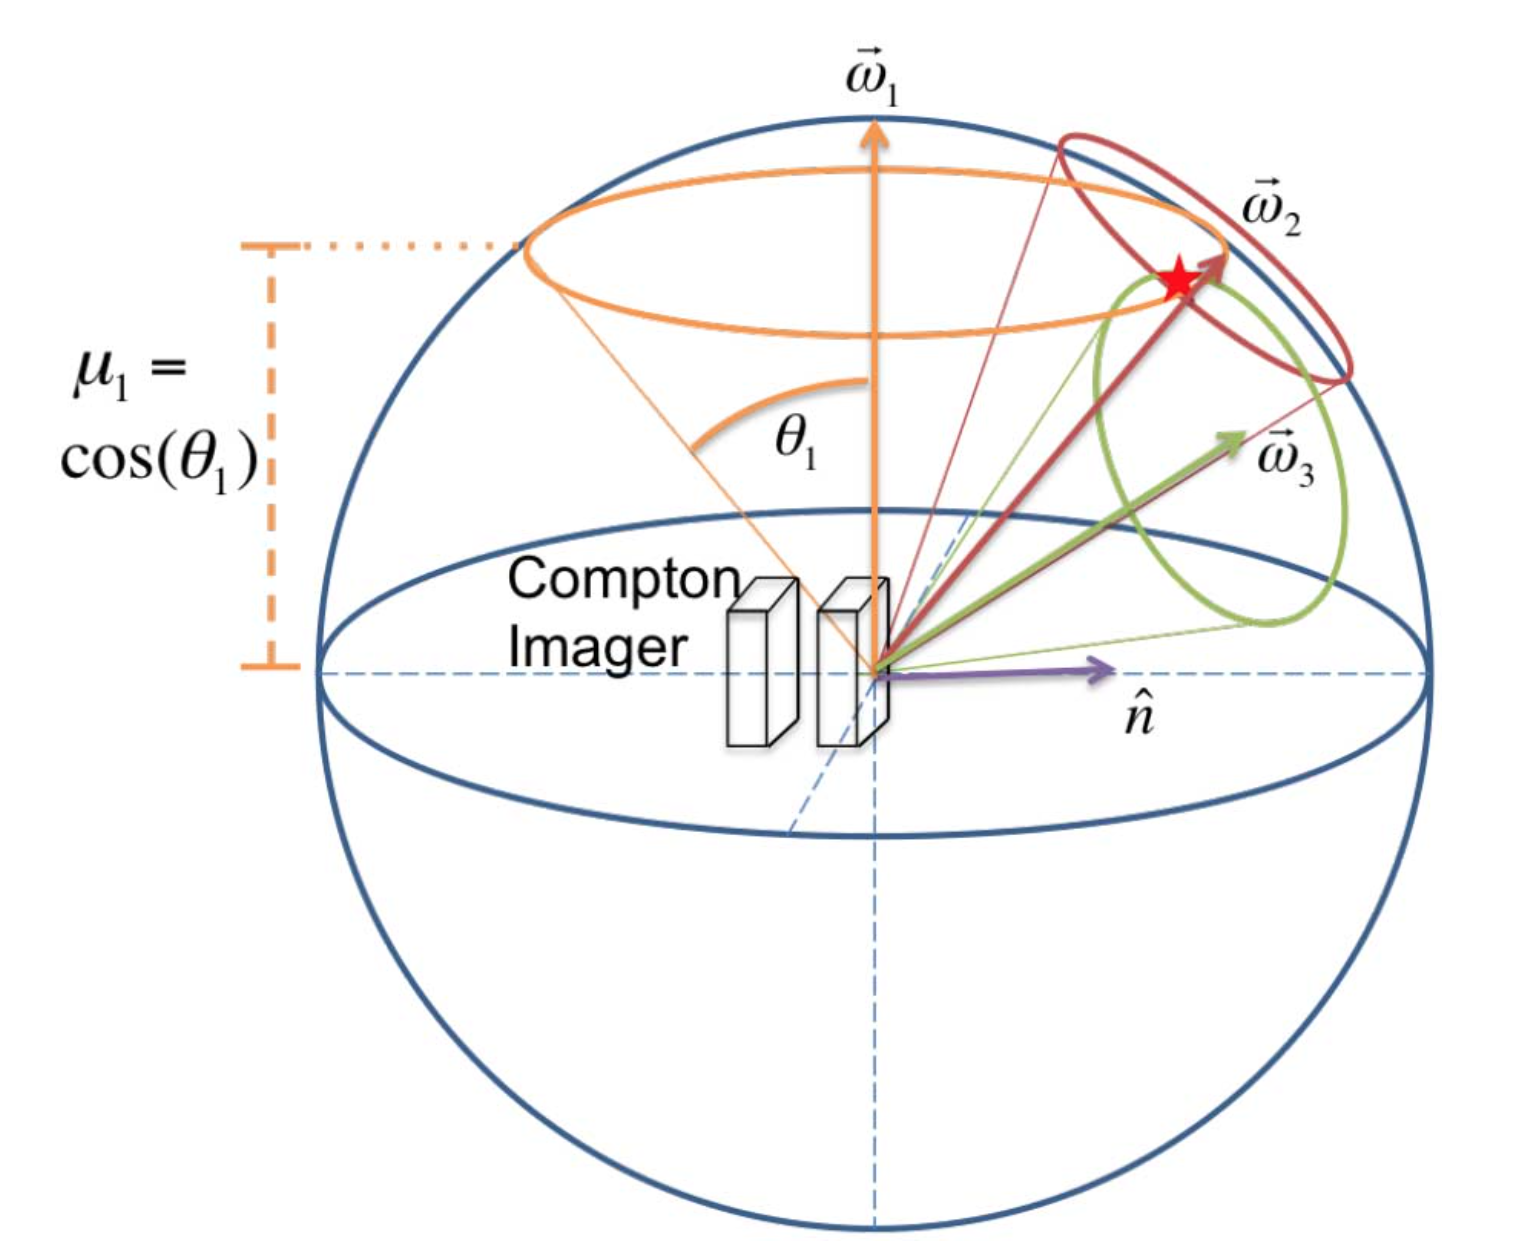
\includegraphics[height=1.7in]{Figures/Compton2.png} & 
\end{tabular}
\end{figure}

Kinematics of correctly sequenced multi-site events define a cone of possible source directions. Cones back-projected into $\mathbb{R}^3$ (3D) or $\mathbb{S}^2$ (2D).

\vspace{-20pt}

\begin{wrapfigure}{R}{0.35\textwidth}
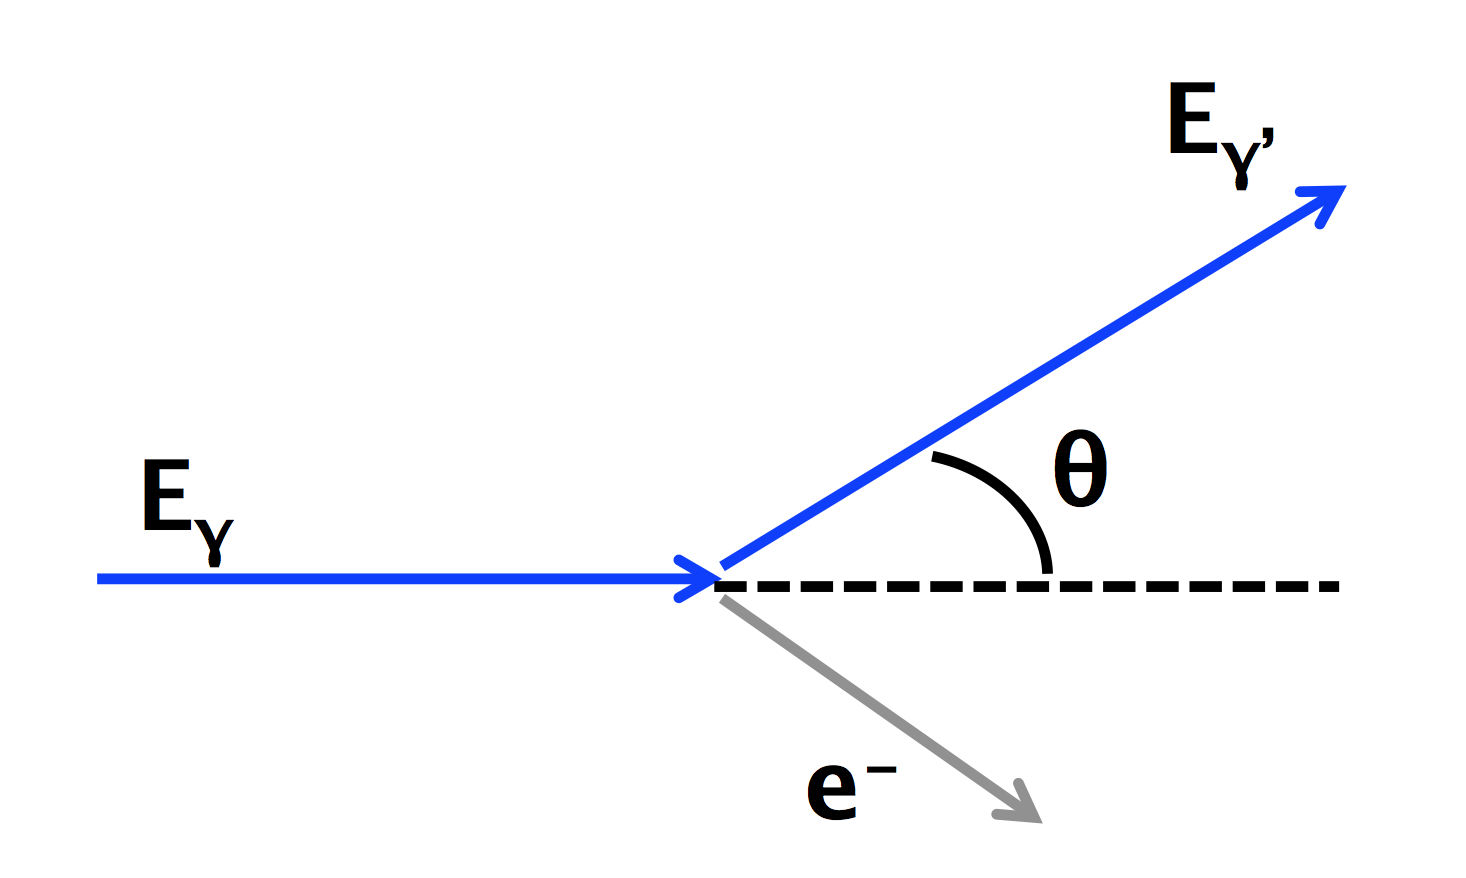
\includegraphics[width=1.2in]{Figures/ComptonKinematic.png} 
\end{wrapfigure}

\hfill\textcolor{white}{a}

\begin{align*}
\mu = \cos(\theta) = 1 + \frac{m_e c^2}{E_\gamma} - \frac{m_e c^2}{E_\gamma^\prime}
\end{align*}

\end{frame}



%------------------------------------------------------------------------------------------------------
\begin{frame}{Compton Imaging - Image Recon.}

Provide each cone with a width and intensity described by a Gaussian function to avoid pixellation effects. Sum $n$ cones together to produce back-projection image \cite{Haefner}

\begin{align*}
b(\hat{\vec{x}}) = \sum_{i=1}^n \frac{w_i}{\sigma_i \sqrt{2\pi}} \exp\left( -\frac{(\hat{\vec{x}} \cdot \hat{\vec{\omega}} - \mu_i)^2}{2\sigma_i^2} \right)\
\end{align*}

\begin{itemize}
\small
\item[-] $\hat{\vec{x}}$ is the unit vector to image pixel
\item[-] $\hat{\vec{\omega}}$ is the unit vector cone axis
\item[-] $\mu$ is the cosine of the scattering angle
\item[-] $w$ is the cone weight (from Klein-Nishina and lever arm distance)
\item[-] $\sigma$ is the cone width (smaller than expected resolution)
\end{itemize}

\end{frame}



%------------------------------------------------------------------------------------------------------
\begin{frame}{PRISM}

\begin{itemize}
\item Multimodal active planar imagers exist (HEMI \cite{Galloway}) $\rightarrow$ suffer from \textbf{limited field-of-view}, especially in coded aperture mode. 
\item Rearrange into a spherical configuration to facilitate 4$\pi$ imaging.
\end{itemize}

\vspace{-10pt}

\begin{figure}
\begin{tabular}{cc}
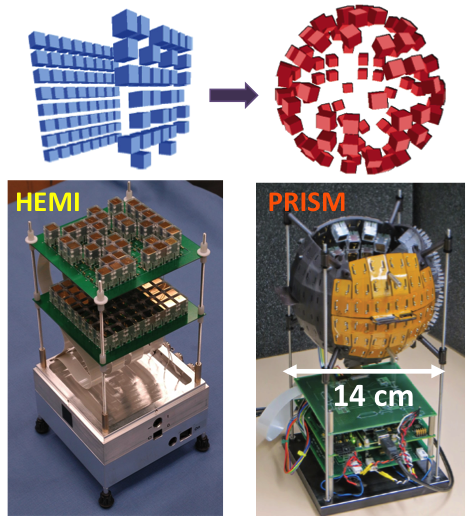
\includegraphics[height=1.6in]{Figures/HEMIvPRISM.png} &
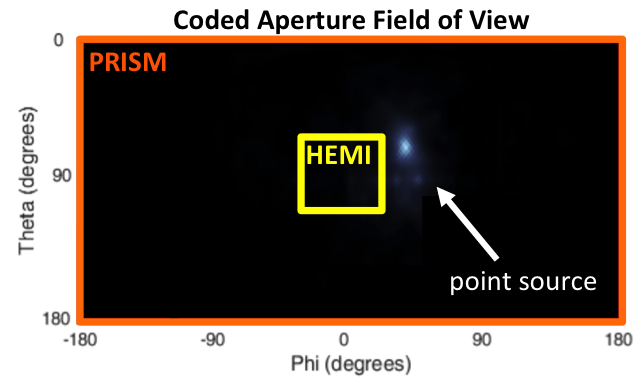
\includegraphics[height=1.4in]{Figures/FOV.png}
\end{tabular}
\end{figure}

\vspace{-15pt}

\begin{wrapfigure}{R}{0.3\textwidth}
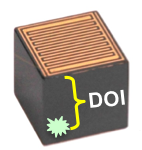
\includegraphics[width=0.5in]{Figures/DOI.png} 
\end{wrapfigure}

\textcolor{white}{a}
\vspace{1pt}

\begin{itemize}
\item 192 available detector locations.
\item Depth-of-interaction (DOI) readout.
\end{itemize}

\end{frame}



%------------------------------------------------------------------------------------------------------
\begin{frame}{Monte Carlo Simulation, Geant4}

Geant4 \cite{Agostinelli} is a \emph{Monte Carlo toolkit} used to simulate the transport of particles through matter.
\begin{itemize}
\small
\item[-] The user writes and compiles their own simulation. % using the Geant4 header files and base framework.
\item[-] \underline{Requires knowledge of C++ and CMake.}
%\item[-] Used heavily in the field of high-energy physics.
\end{itemize}

\begin{figure}
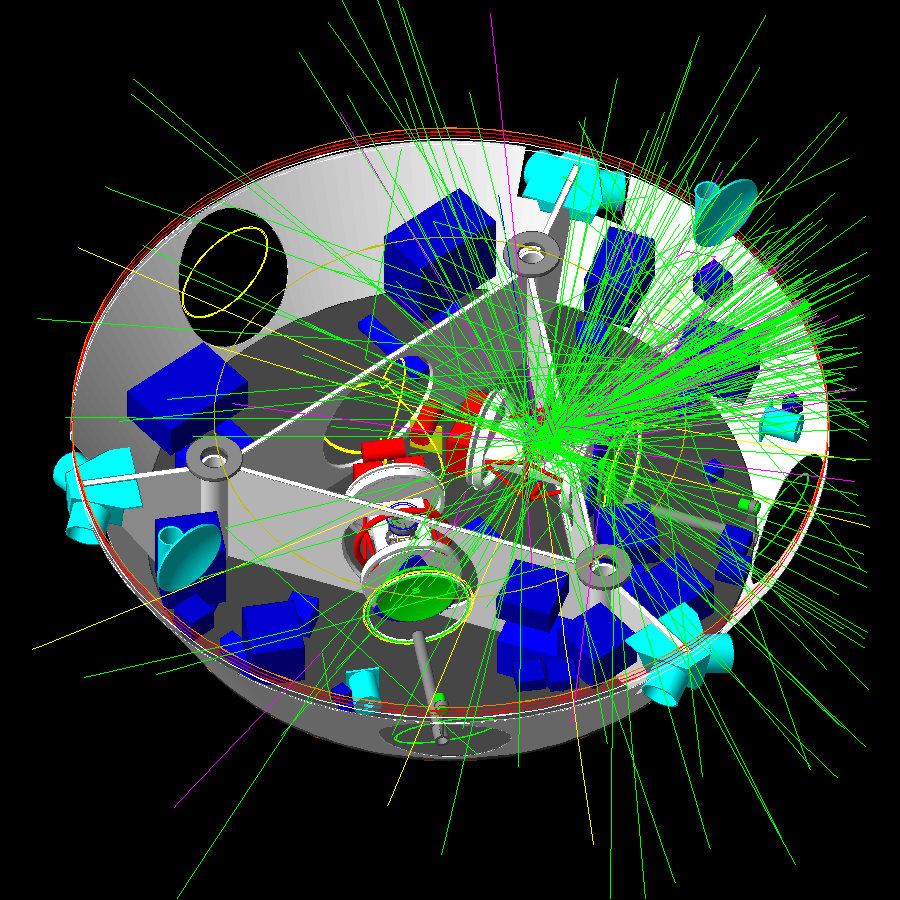
\includegraphics[height=1.4in]{Figures/LISAGeant4.jpg}
\end{figure}

\textcolor{blue}{Simple raytracing simulation was developed over the summer to determine coded aperture system response to far-field point sources.}
%\begin{itemize}
%\small
%\item[-] Raytracing with attenuation
%\end{itemize}

\end{frame}


%------------------------------------------------------------------------------------------------------
\begin{frame}{What did I do?}


\begin{enumerate}\setlength\itemsep{1.3em}
\item Upgraded simulation to include scattering, electron production, multi-interaction tracking, geometry and source modifications. 
\begin{itemize}
\small
\item[-] User interaction via macro files passed to executable
\item[-] Track energy deposition, detector ID, DOI, ...
\item[-] Output to structured binary data files
\end{itemize}
\item Developed Python tools to 
\begin{itemize}
\small
\item[-] Parse output data
\item[-] Perform MLEM coded aperture image reconstruction
\item[-] Collect coincident Compton events and sequence tracks
\item[-] Perform Compton cone back-projection image reconstruction
\end{itemize}
\end{enumerate}



\end{frame}





%------------------------------------------------------------------------------------------------------
\begin{frame}{2D Coded Aperture System Response}

Simulate far-field point sources (parallel rays at infinity) at each image pixel in 4$\pi$.
\begin{itemize}
\small
\item[-] \emph{Hierarchical Equal Area isoLatitude Pixelization} (HEALPix) \cite{Gorski} discretization of a sphere with 3072 pixels.
\end{itemize}

\begin{figure}
\centering
\begin{tabular}{m{0.3\linewidth} m{0.3\linewidth}}
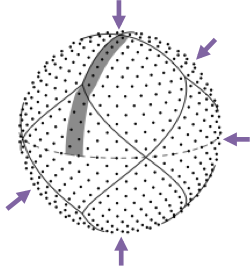
\includegraphics[height=1.2in]{Figures/Healpix.png} &
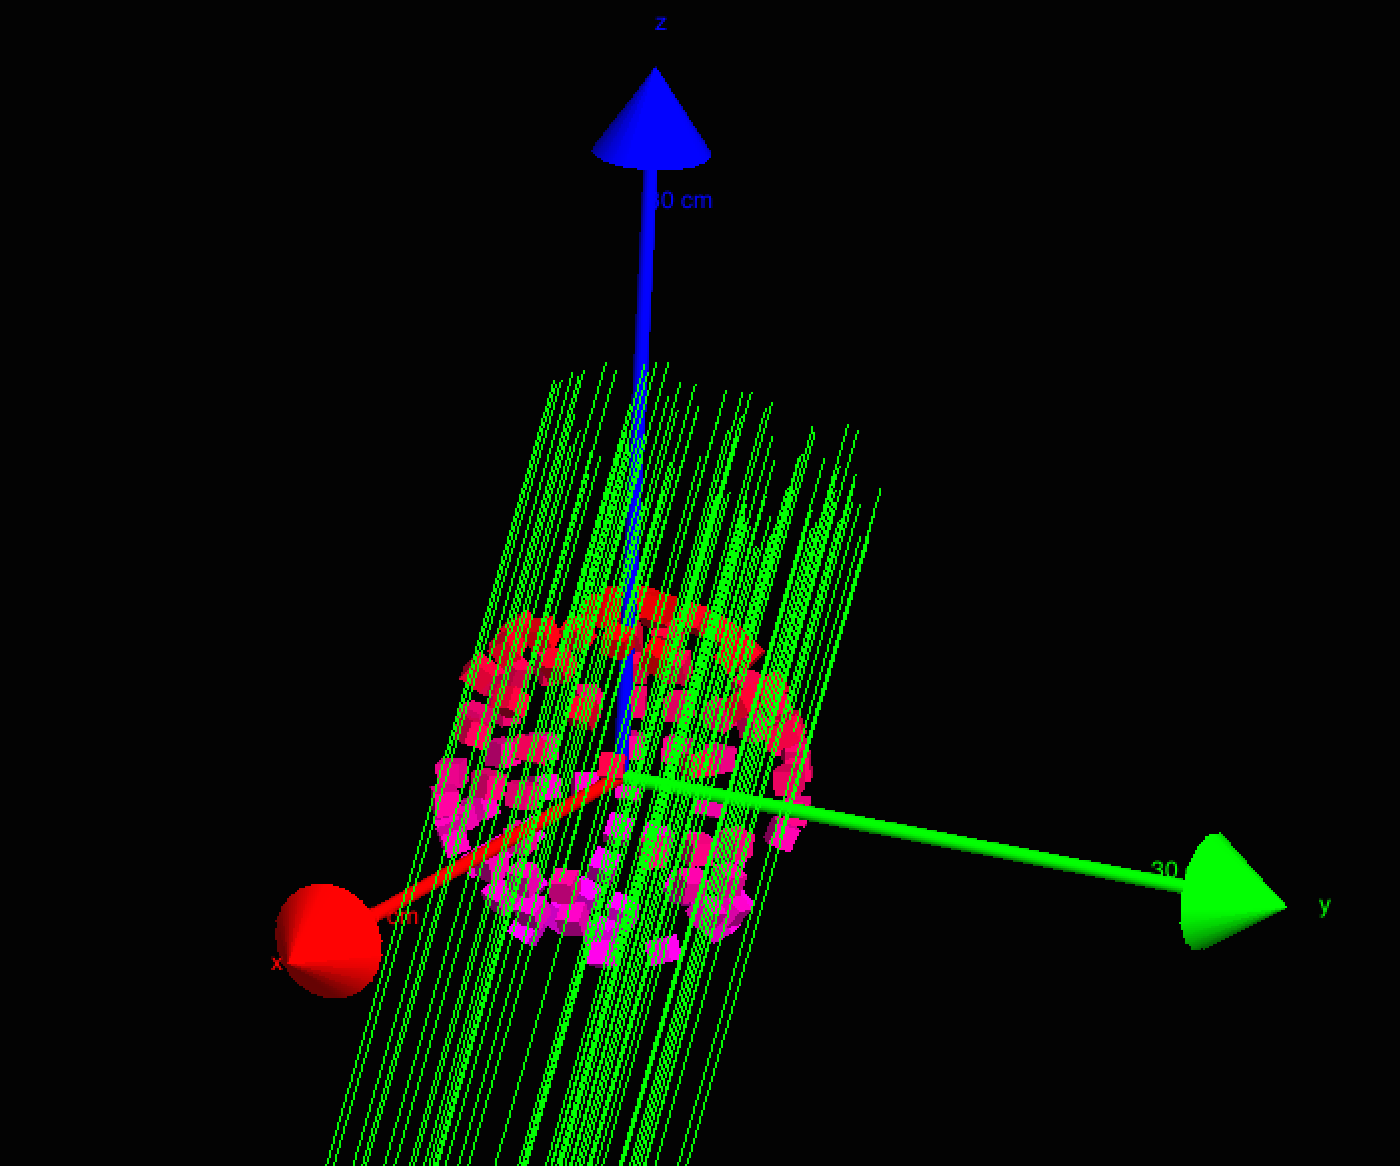
\includegraphics[height=1.8in]{Figures/FarFieldVis2.png}
\end{tabular}
\end{figure}

\end{frame}



%------------------------------------------------------------------------------------------------------
\begin{frame}{2D Coded Aperture System Response}

\textbf{Random mask}\\ [1ex]
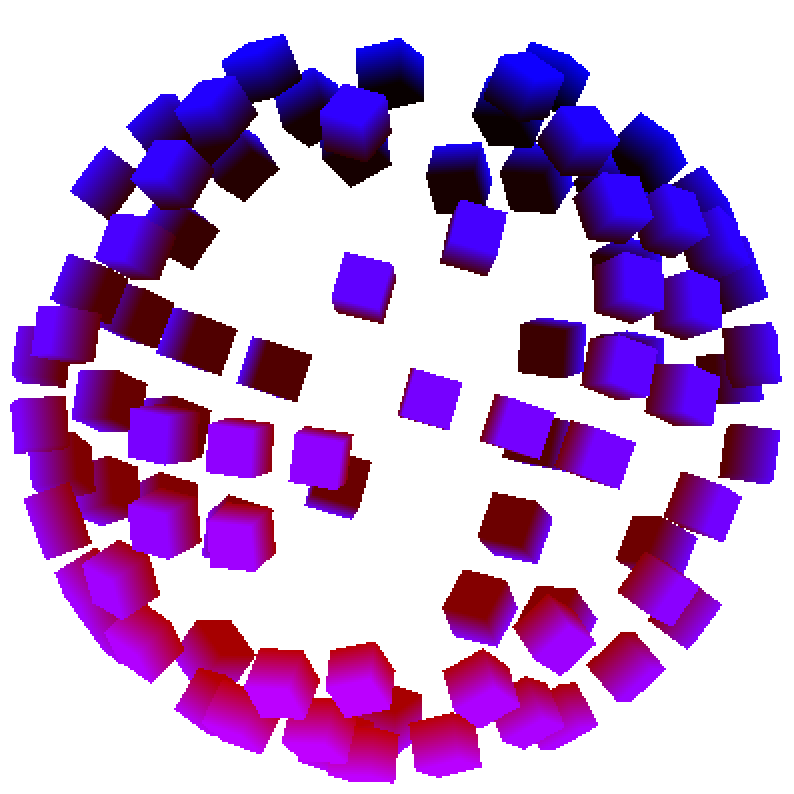
\includegraphics[height=35pt, width=35pt]{Figures/RandMask.png}

\vspace{-60pt}
\begin{figure}
\begin{tabular}{m{0.12\linewidth} m{0.4\linewidth} m{0.4\linewidth}}
	& Without DOI 
\includegraphics[height=0.4in]{Figures/noDOI.png} & 
	With DOI 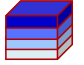
\includegraphics[height=0.4in]{Figures/DOIbins.png} \\
	\small{60 keV} & 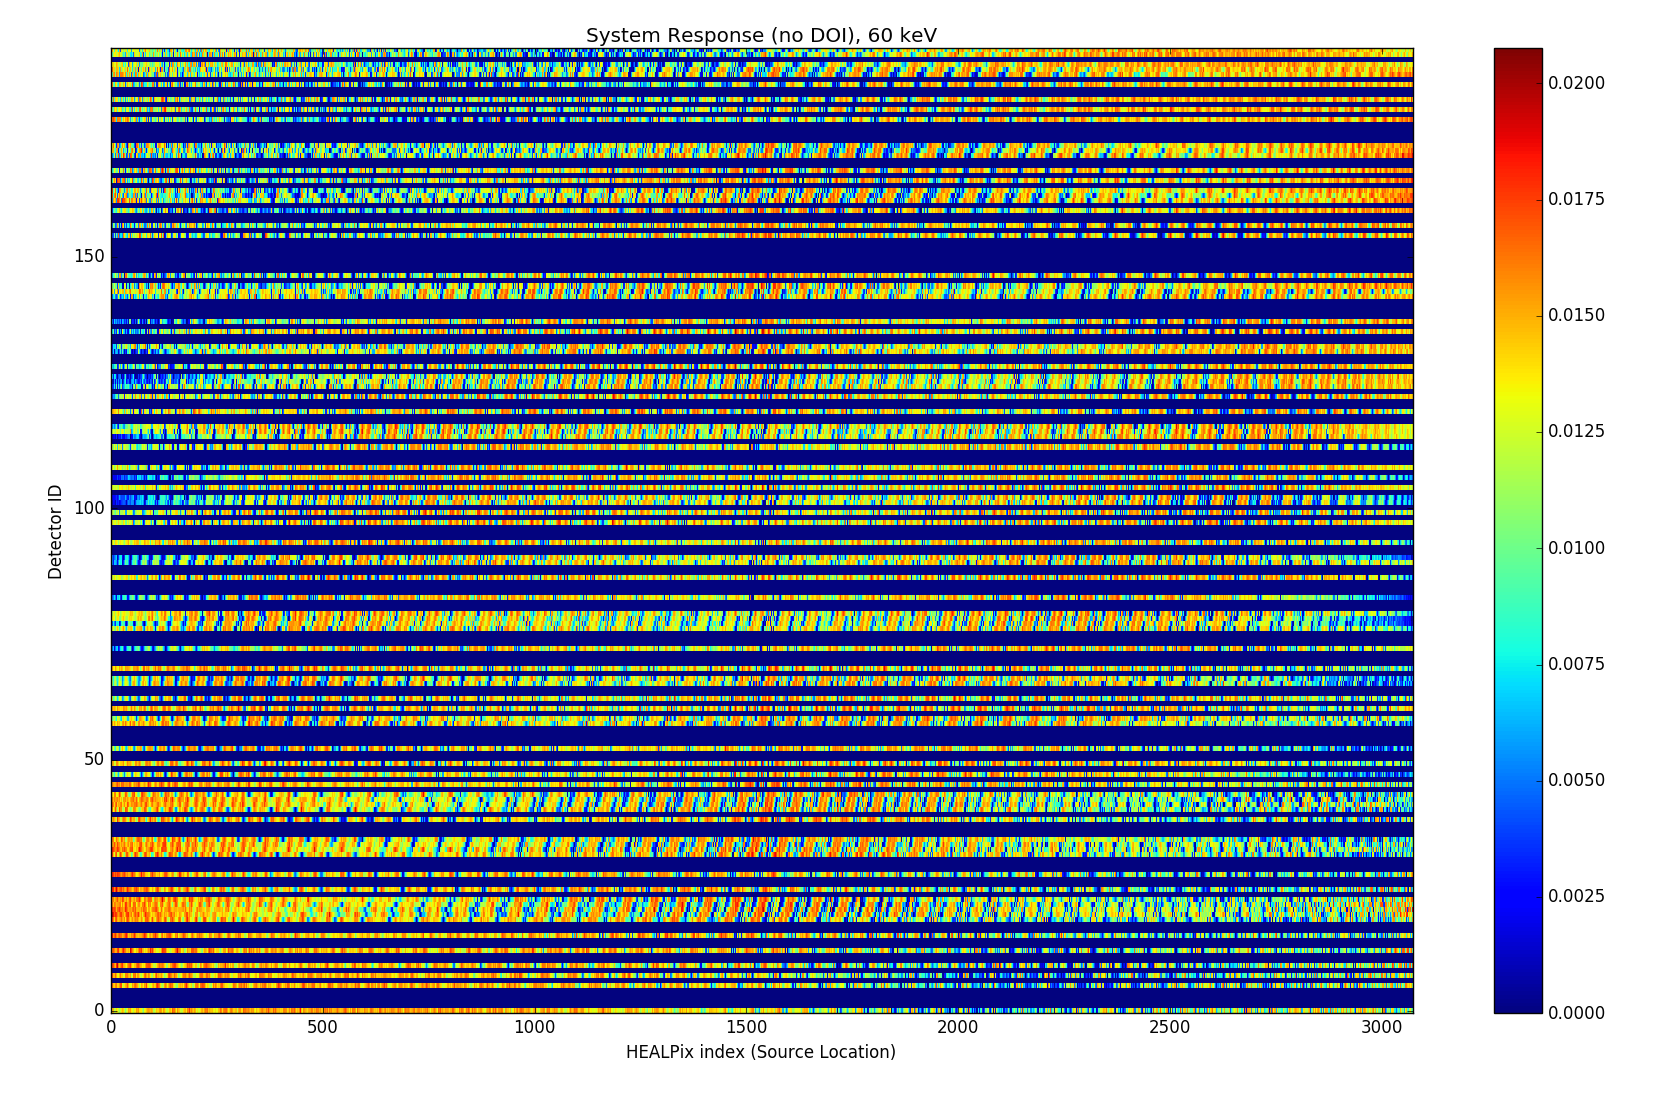
\includegraphics[height=85pt]{Figures/SystemResponse_60_noDOI.png} & 
	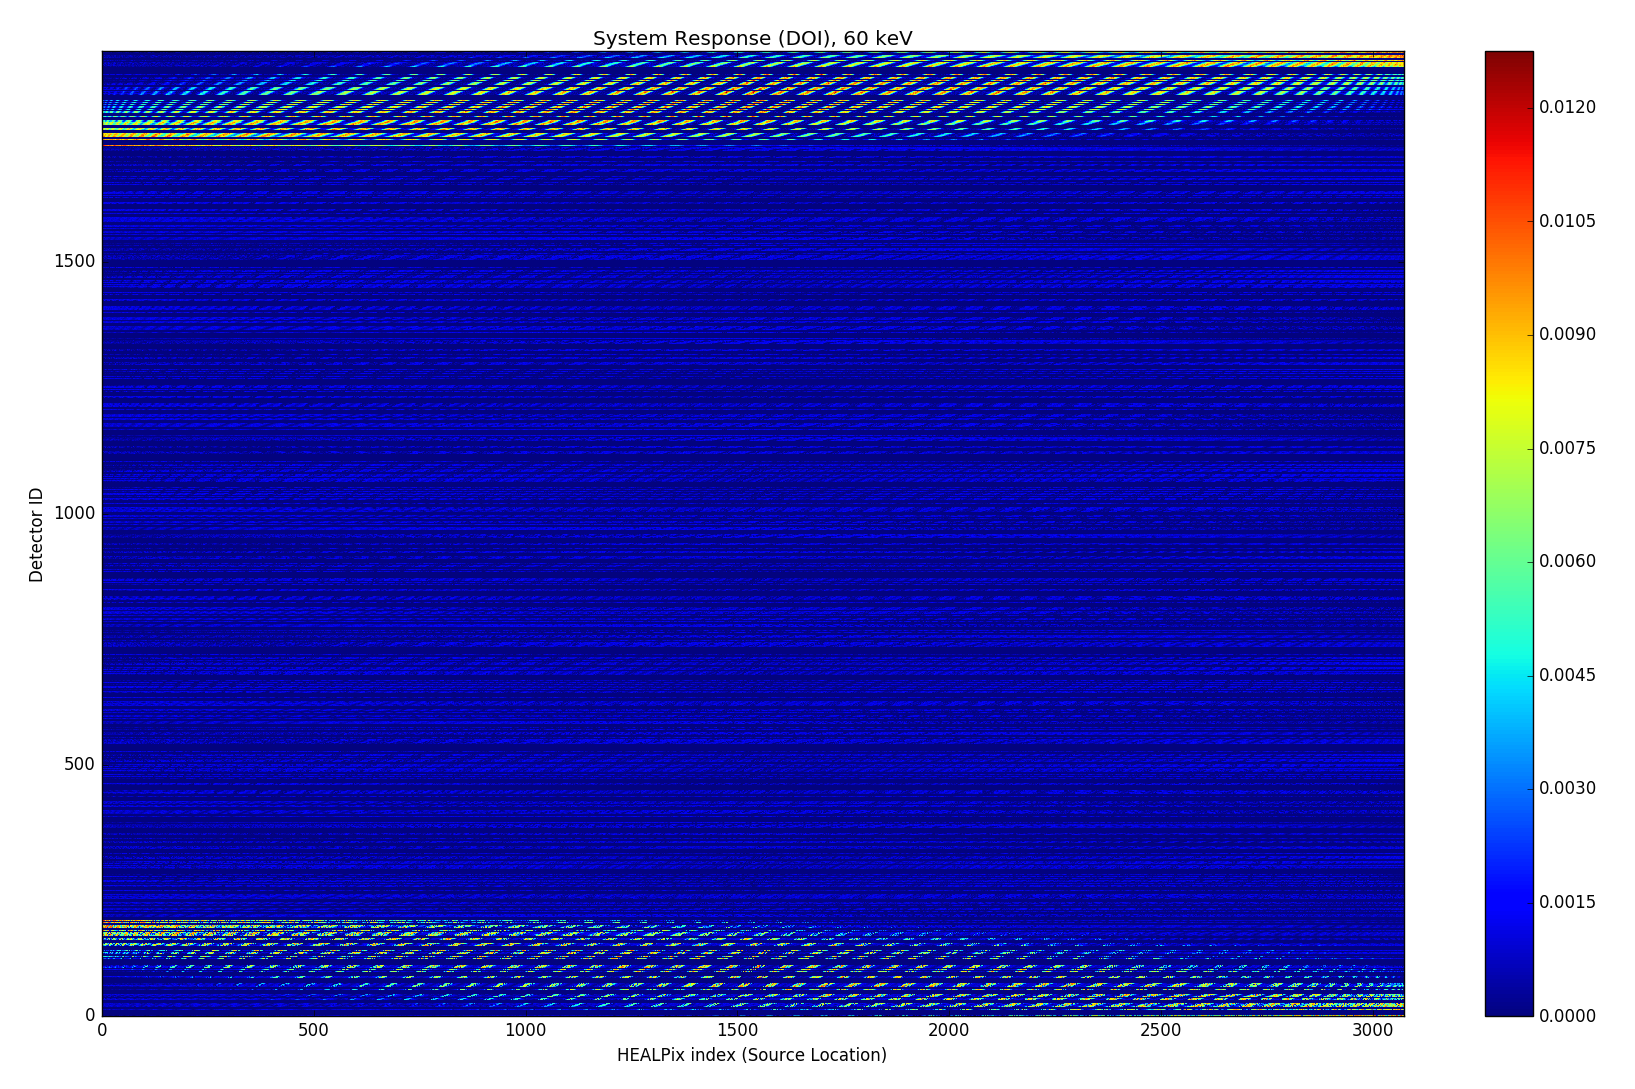
\includegraphics[height=85pt]{Figures/SystemResponse_60_DOI.png} \\ 
	\small{186 keV} & 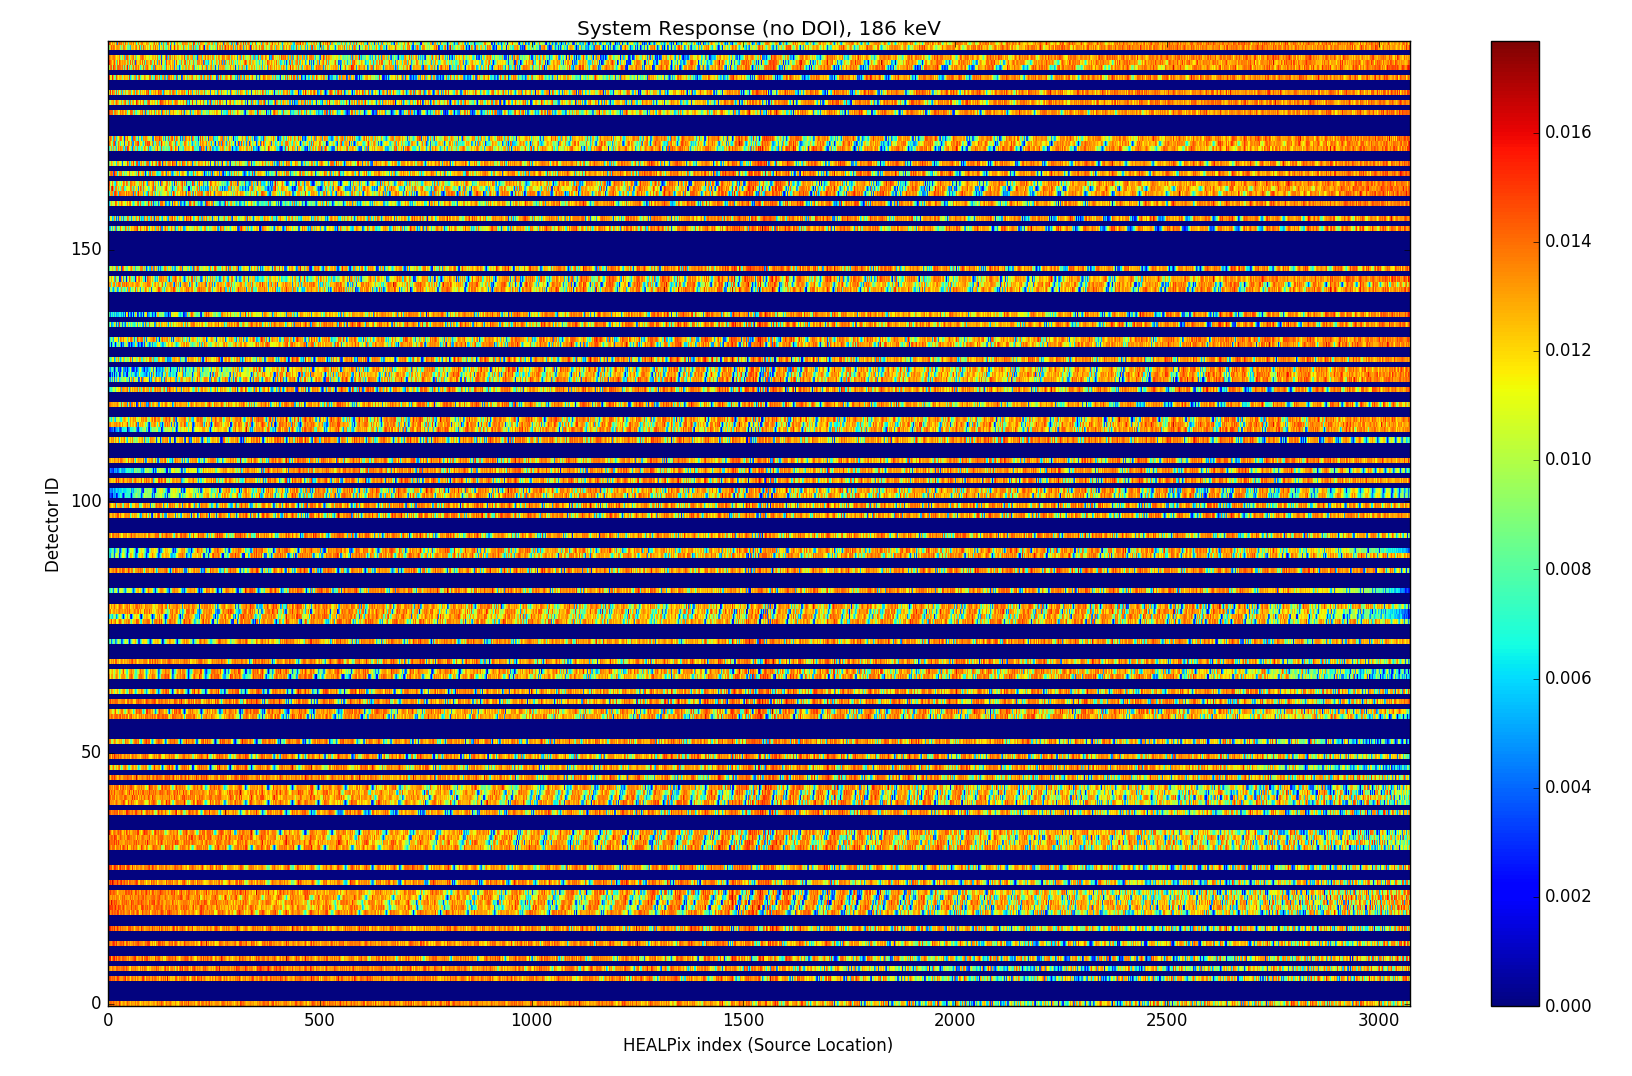
\includegraphics[height=85pt]{Figures/SystemResponse_186_noDOI.png} & 
	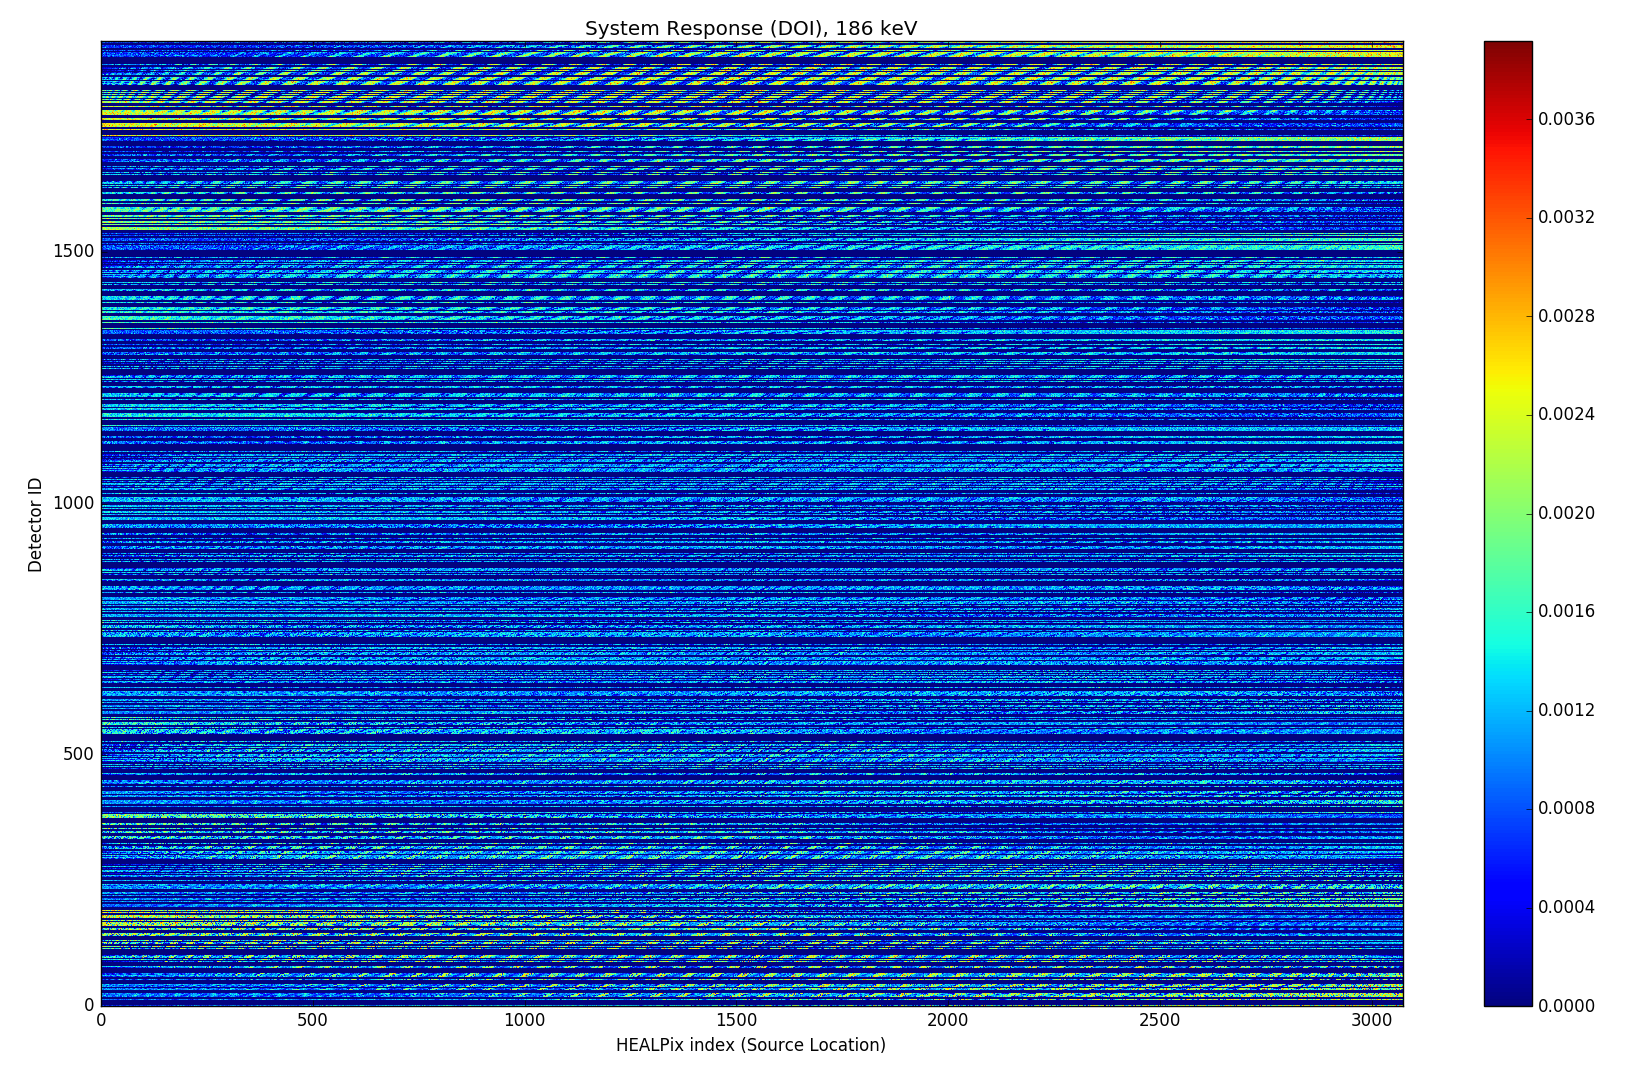
\includegraphics[height=85pt]{Figures/SystemResponse_186_DOI.png}
\end{tabular}
\end{figure}


\end{frame}




%------------------------------------------------------------------------------------------------------
\begin{frame}{MLEM Images}

\textbf{60 keV, random mask}\\ [1ex]
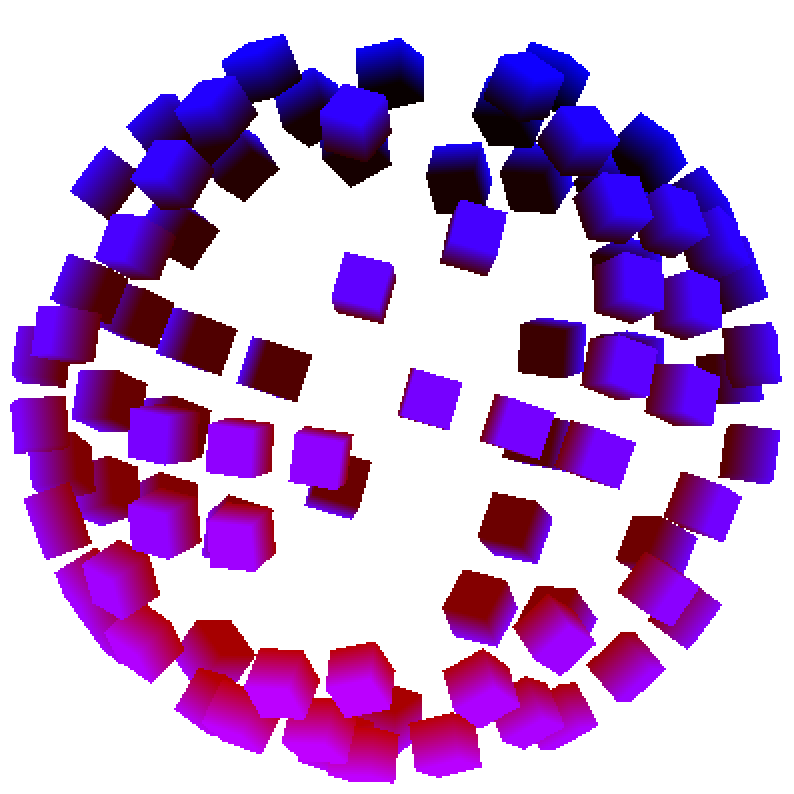
\includegraphics[height=35pt, width=35pt]{Figures/RandMask.png}

\vspace{-40pt}
\begin{figure}
\begin{tabular}{m{0.12\linewidth} m{0.4\linewidth} m{0.4\linewidth}}
	& 10 iterations & 30 iterations \\
	Without DOI & 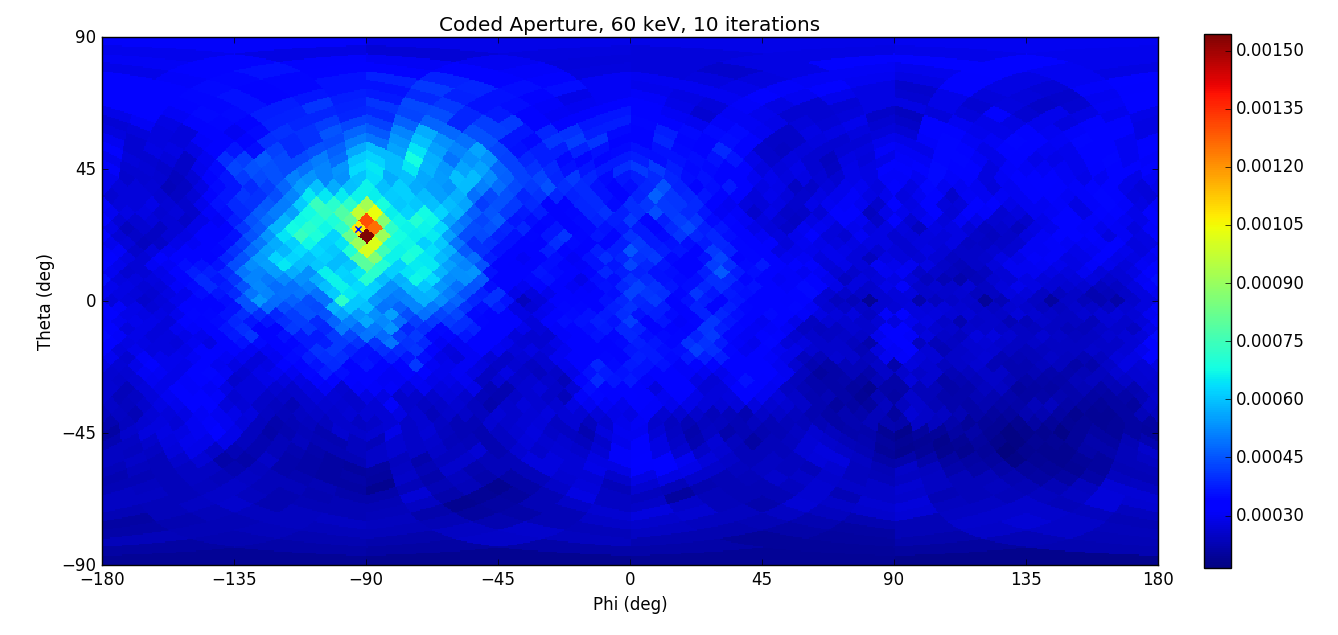
\includegraphics[height=75pt, width=135pt]{Figures/MLEM_60_noDOI_HP912_10itr.png} & 
	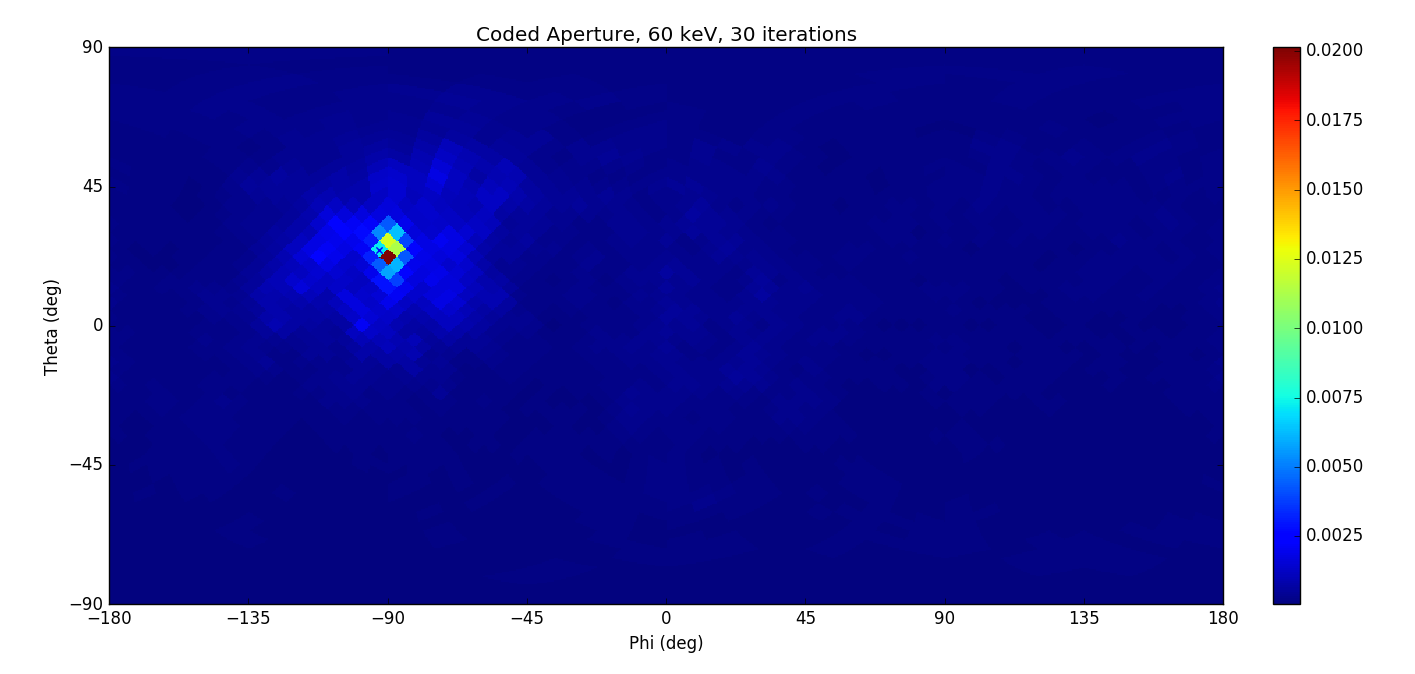
\includegraphics[height=75pt, width=135pt]{Figures/MLEM_60_noDOI_HP912_30itr.png} \\
	With DOI (inner) & 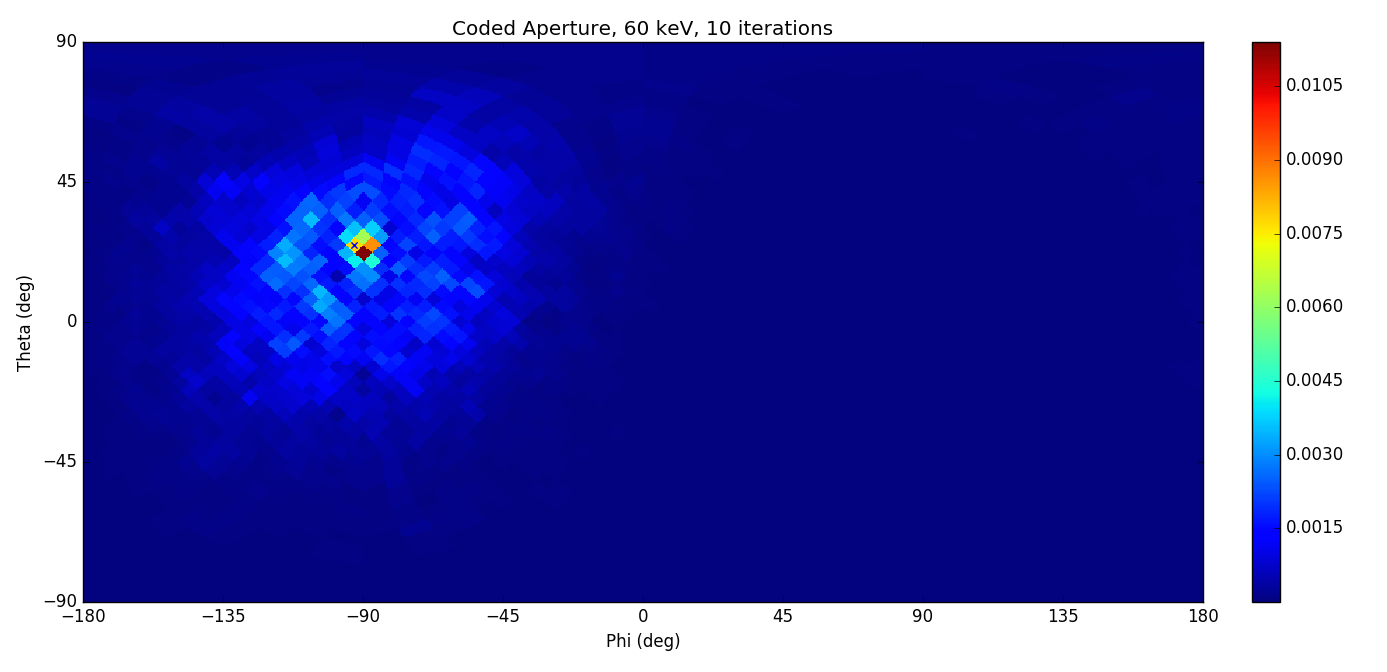
\includegraphics[height=75pt, width=135pt]{Figures/MLEM_60_DOI_HP912_10itr.png} & 
	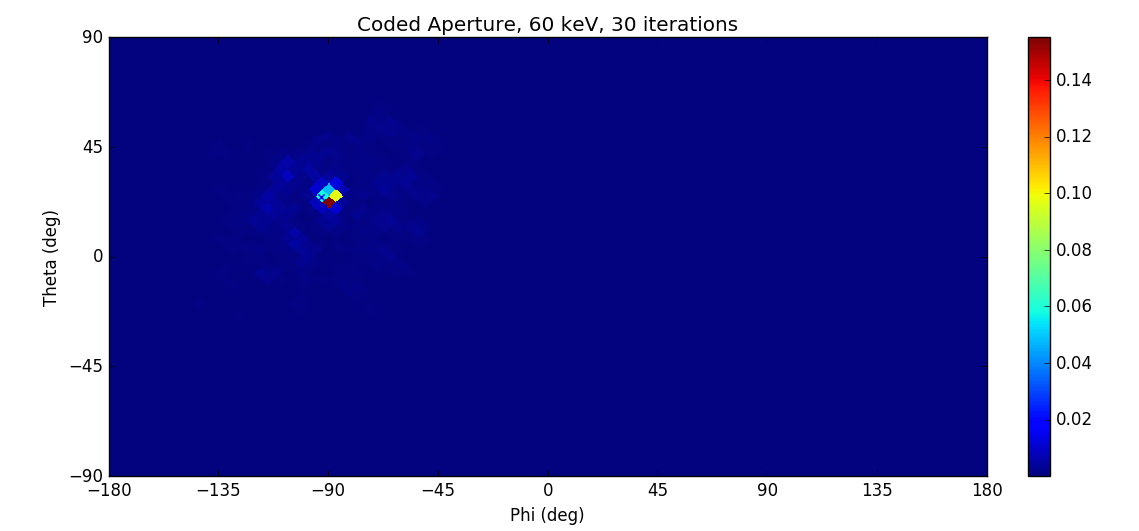
\includegraphics[height=75pt, width=135pt]{Figures/MLEM_60_DOI_HP912_30itr.png}
\end{tabular}
\end{figure}

\end{frame}



%------------------------------------------------------------------------------------------------------
\begin{frame}{Compton Cone Back-Projection Images}

\textbf{Fully populated mask, 2-interaction sequences}\\ [1ex]
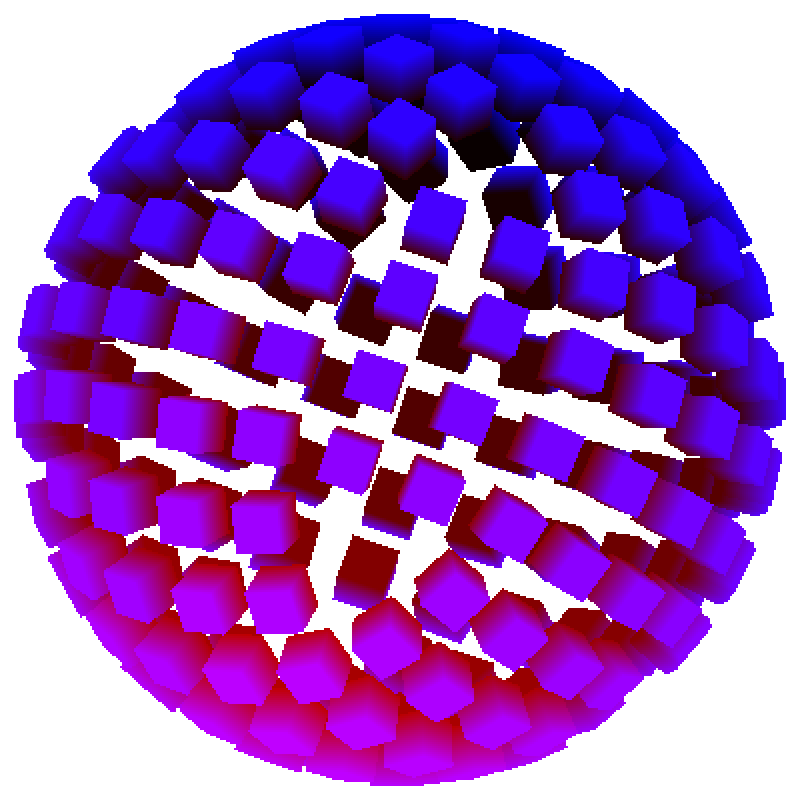
\includegraphics[height=35pt, width=35pt]{Figures/FullMask.png}

\vspace{-35pt}
\begin{figure}
\begin{tabular}{m{0.11\linewidth} m{0.4\linewidth} m{0.4\linewidth}}
	& 200 keV & 662 keV \\
	50 cones & 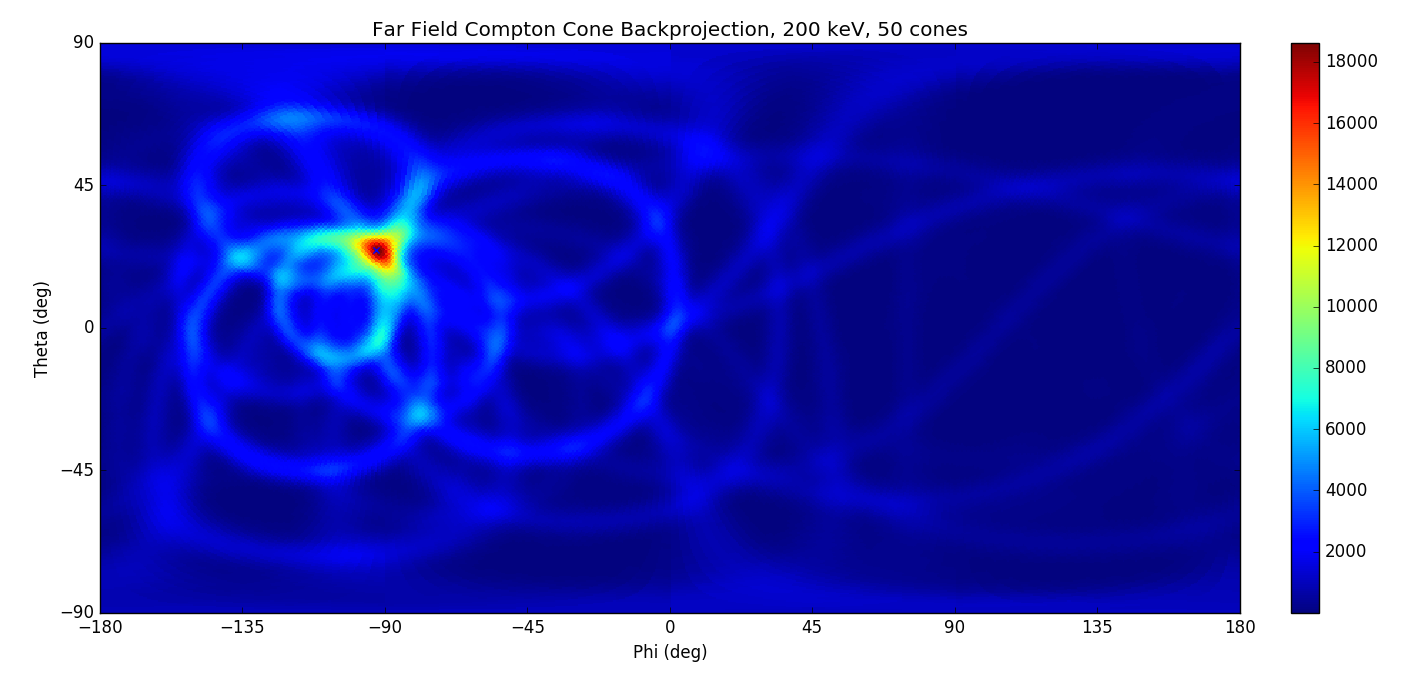
\includegraphics[height=75pt, width=135pt]{Figures/Compton_200_50cones.png} & 
	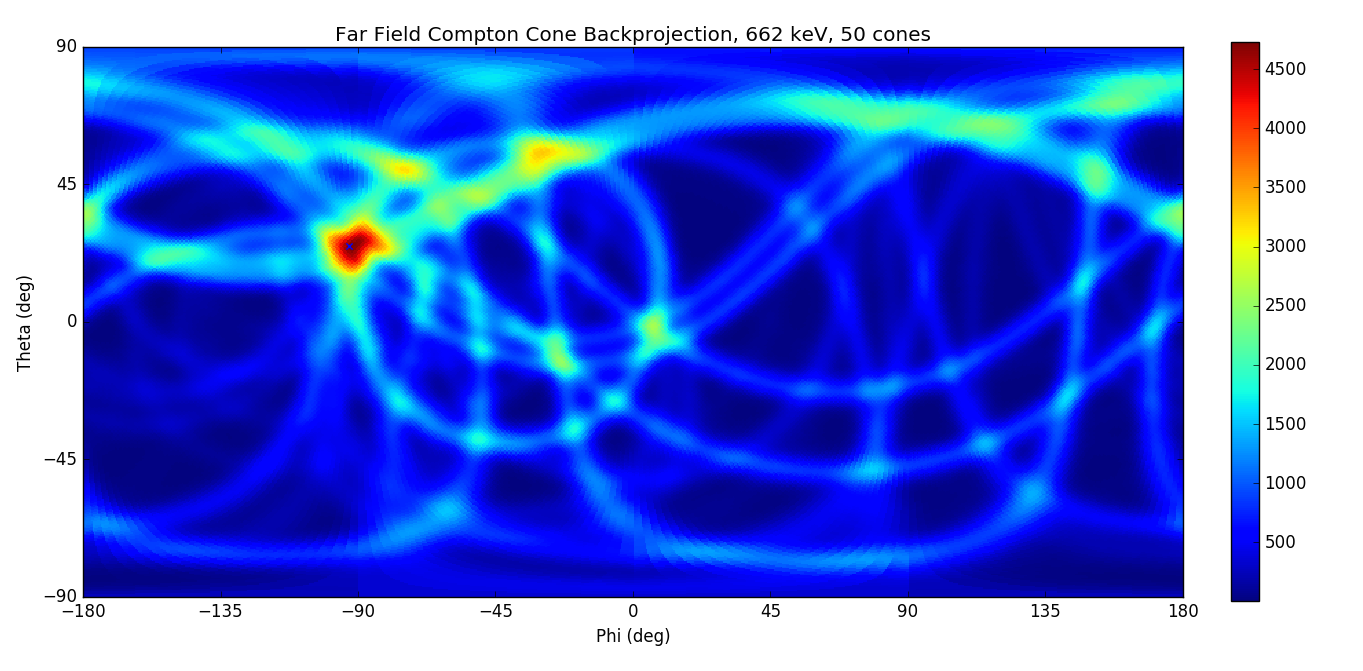
\includegraphics[height=75pt, width=135pt]{Figures/Compton_662_50cones.png} \\
	2000 cones & 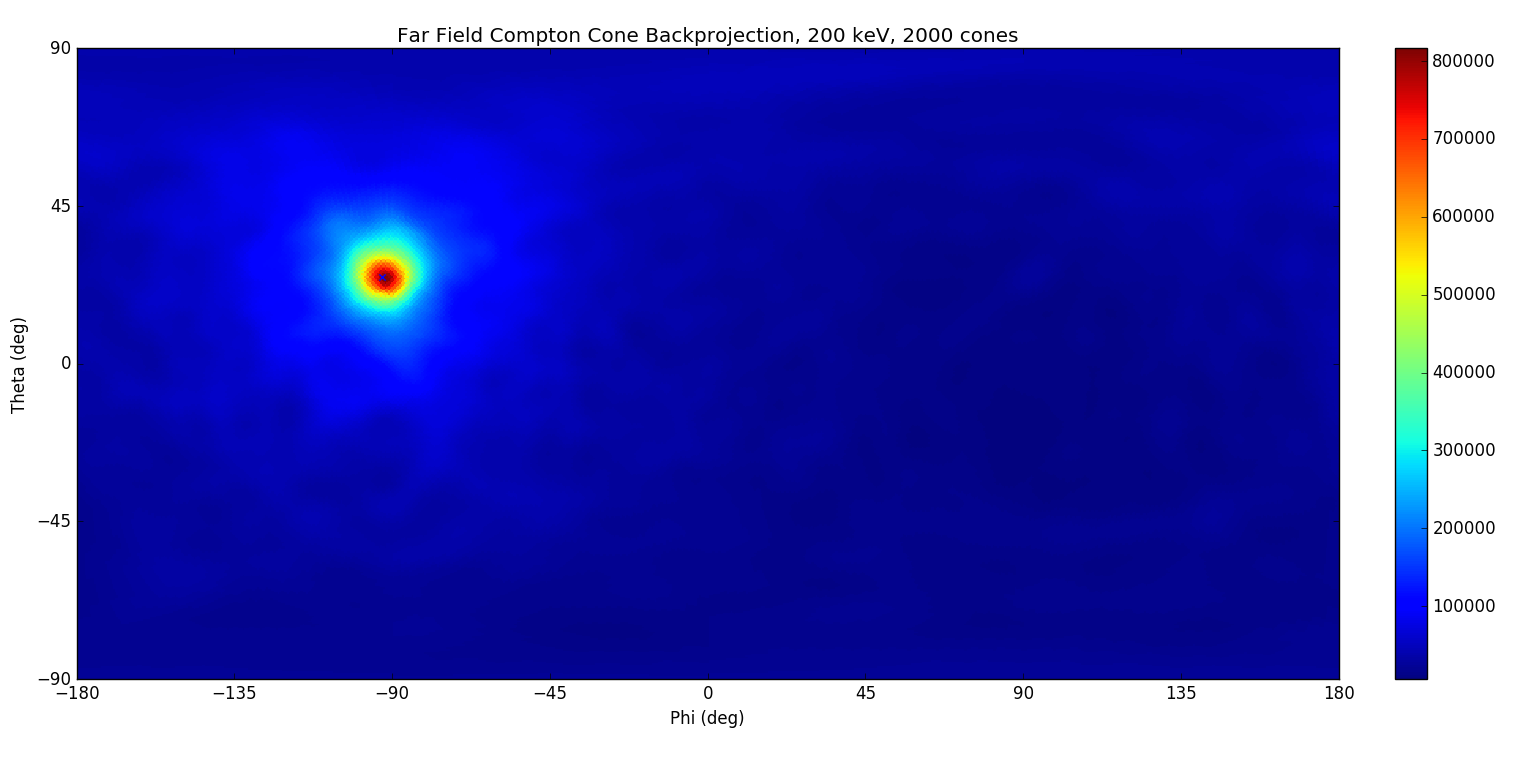
\includegraphics[height=75pt, width=135pt]{Figures/Compton_200_2000cones.png} & 
	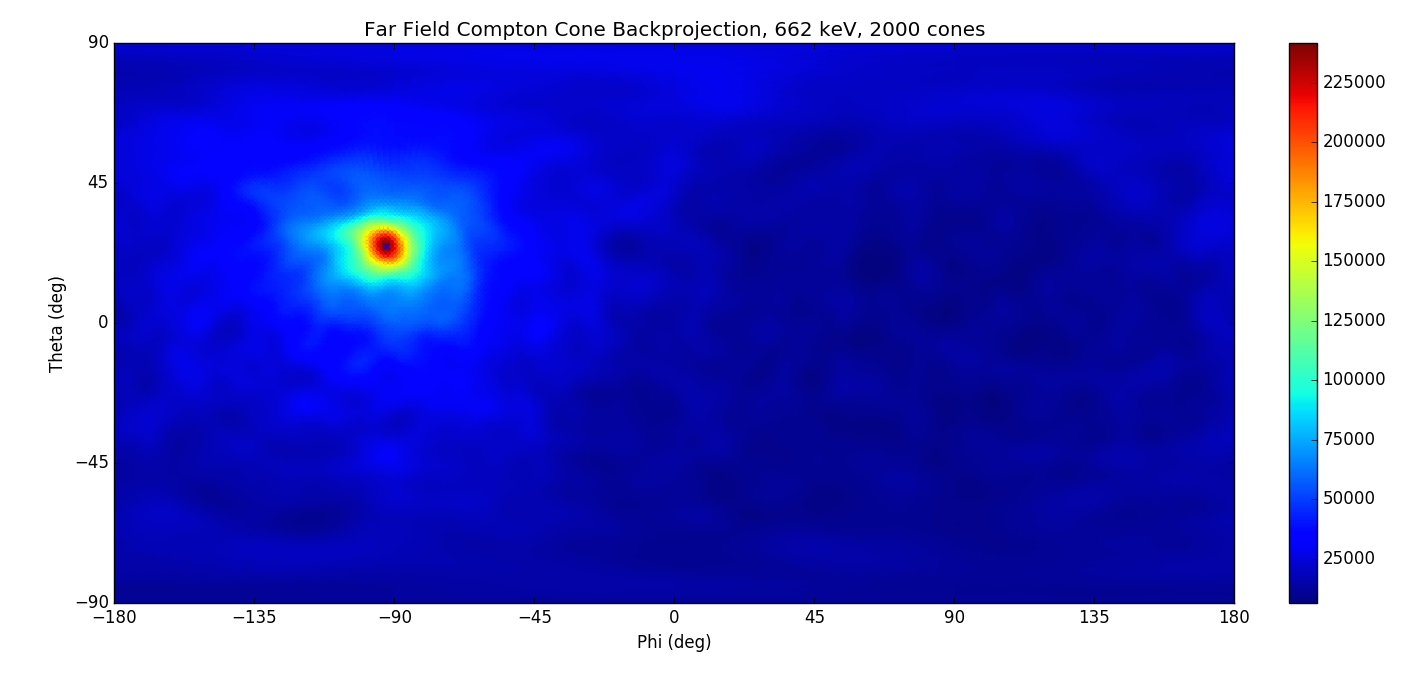
\includegraphics[height=75pt, width=135pt]{Figures/Compton_662_2000cones.png}
\end{tabular}
\end{figure}

\end{frame}



%------------------------------------------------------------------------------------------------------
\begin{frame}{Far-Field Ring Source}

\vspace{-2ex}
\begin{figure}
\begin{tabular}{cc}
	\textbf{Coded Aperture} & \textbf{Compton Imaging} \\
	60 keV, inner DOI, 50 itr & 662 keV, without DOI \\
	Random mask & Full mask \\
	$1.0\times10^5$ total counts & $2.2 \times10^4$ cones \\
	&\\
	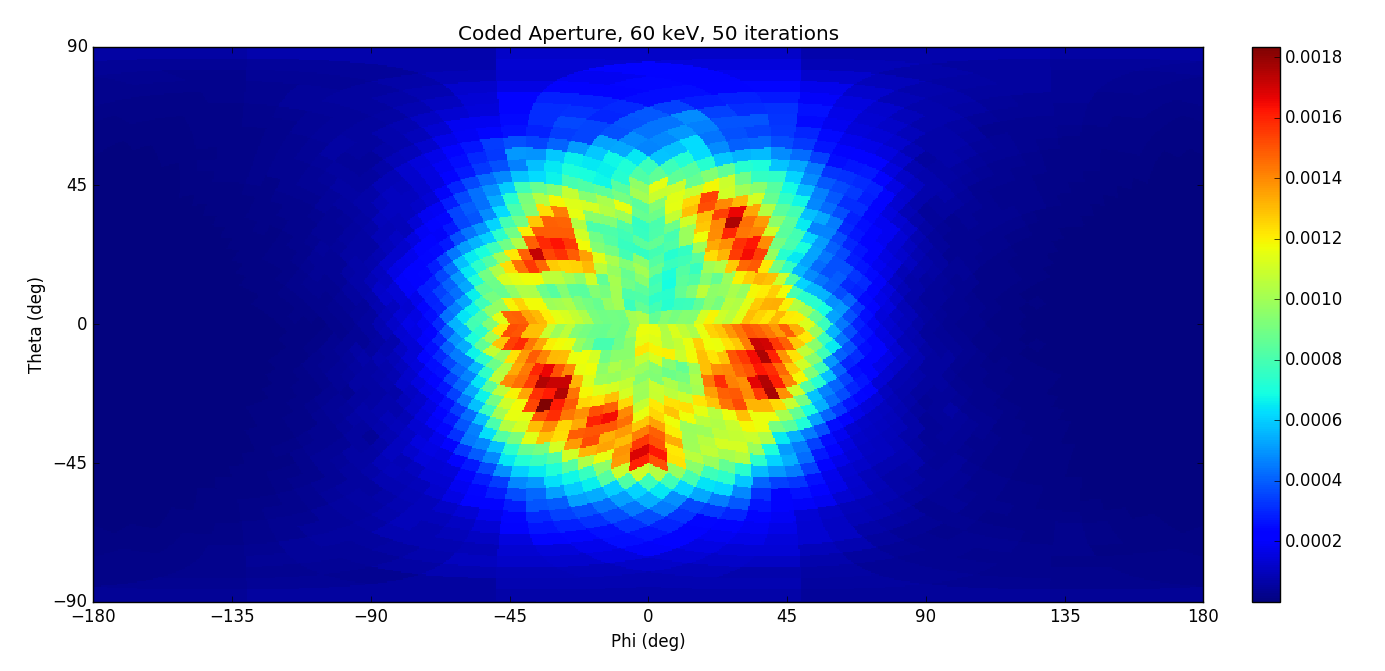
\includegraphics[height=80pt, width=160pt]{Figures/FarfieldRing_60_DOI.png} & 
	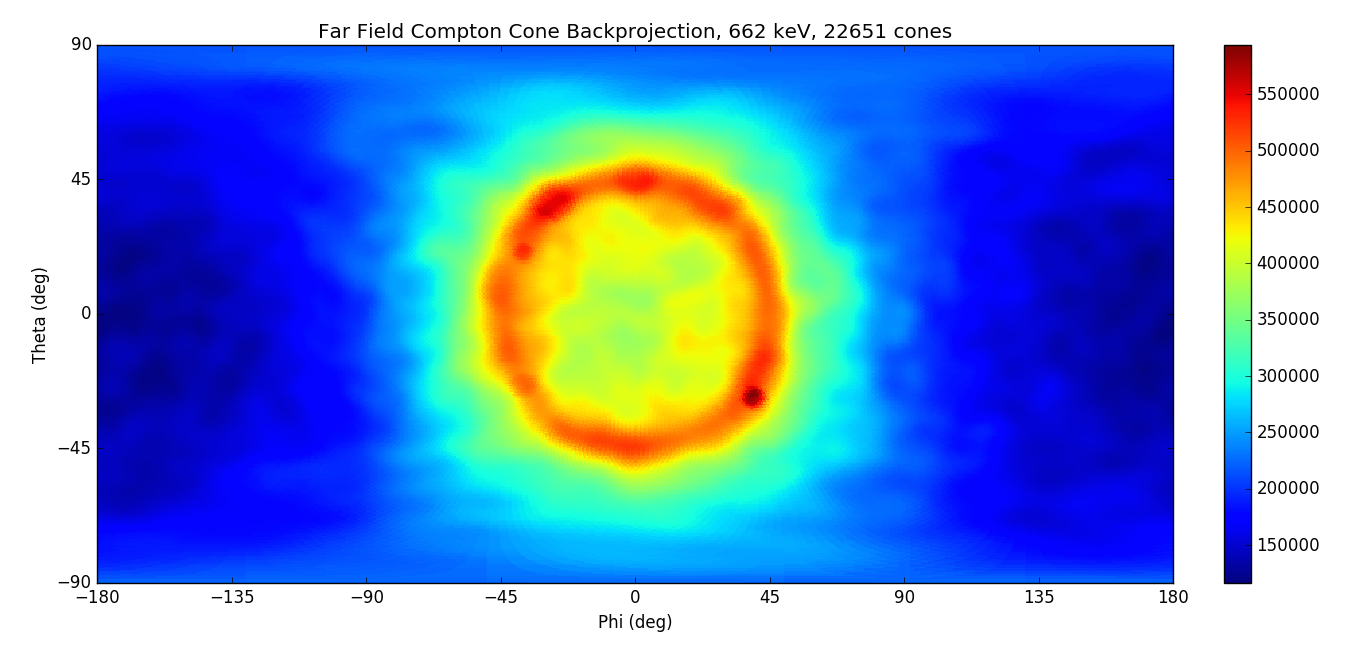
\includegraphics[height=80pt, width=160pt]{Figures/FarfieldRing_662.png} \\
	%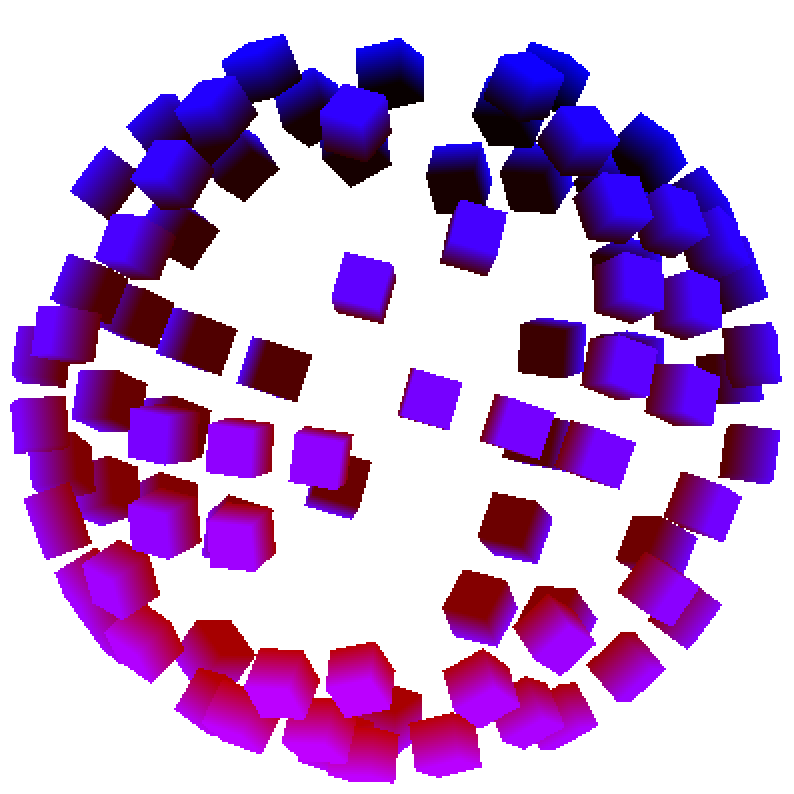
\includegraphics[height=50pt, width=50pt]{Figures/RandMask.png} & 
	%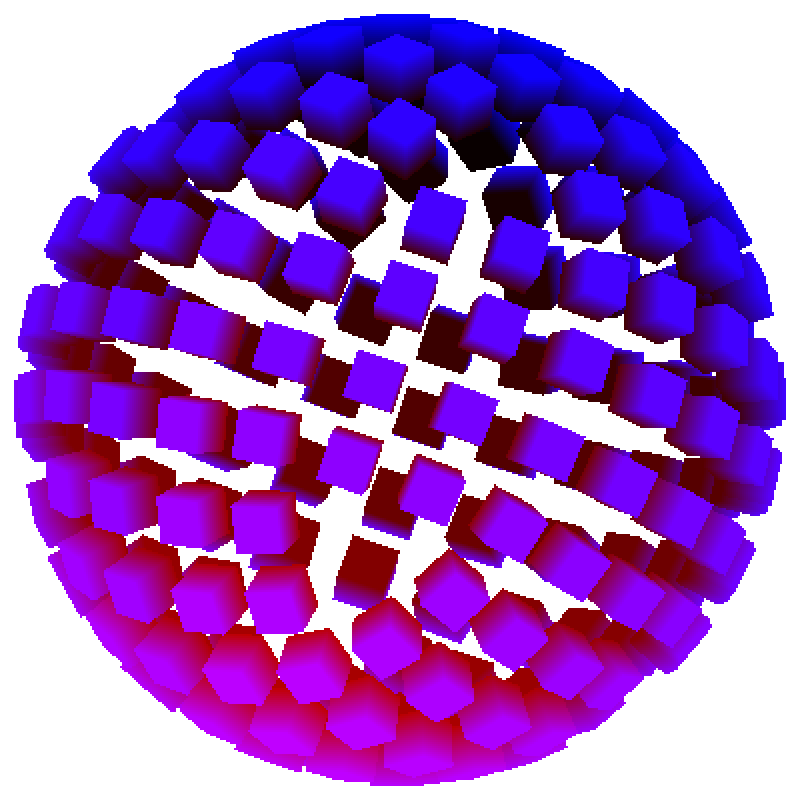
\includegraphics[height=50pt, width=50pt]{Figures/FullMask.png}
\end{tabular}
\end{figure}

\end{frame}



%------------------------------------------------------------------------------------------------------
\begin{frame}{Conclusions/Future Work}

\begin{itemize}
\item PRISM is a handheld, broad energy sensitive, high efficiency gamma-ray imager with a multi-modal 4$\pi$ FOV.
\item Geant4 simulation was upgraded. % to include more relevant physics and data collection, as well as geometry and source modification features.
\item Reconstruction code was written and tested. %for coded aperture and Compton imaging reconstruction.
\item Test reconstructions behaved as expected.  %as a function of energy, iterations, DOI, and number of cones. 
%\item Demonstration of 4$\pi$ imaging concept with spherical CZT based gamma-ray imager and have laid the groundwork for further analysis.
\end{itemize}

\vspace{2ex}

\textbf{Future Work}
\begin{itemize}
\small
\item[$\circ$] Multiple point sources, near-field sources, distributed sources.
\item[$\circ$] List-mode MLEM.
\item[$\circ$] $>2$ interaction Compton sequencing.
\item[$\circ$] Static 3D imaging, 3D tomographic motion imaging.
\item[$\circ$] Real-time imaging, fused with contextual sensors (RGB, LiDAR) \cite{Barnowski}.
\item[$\circ$] Detection efficiency, charge collection, coincidence gating.
\item[$\circ$] ...
\end{itemize}

\end{frame}



%------------------------------------------------------------------------------------------------------
\begin{frame}[plain,c]

\begin{center}
\Large Questions?
\end{center}

%\includemedia[
%  activate=pageopen,
%  width=200pt,height=170pt,
%  addresource=Figures/ComptonMov.mov,
%  flashvars={%
%src=Figures/ComptonMov.mov
%&scaleMode=stretch}
%]{}{StrobeMediaPlayback.swf}

\end{frame}



%------------------------------------------------------------------------------------------------------
\begin{frame}{References}    
\vspace{-14ex}
\tiny
  \begin{thebibliography}{10}    
  \setbeamertemplate{bibliography item}[text]
   \bibitem{Luke} P. N. Luke, IEEE Trans. Nucl. Sci. 4, 207 (1995).
  \bibitem{Wahl} C. Wahl, Ph.D. Thesis, University of Michigan (2011).
  \bibitem{Fenimore} E. E. Fenimore and T. M. Cannon, Applied Optics 17, 3 (1978).
  \bibitem{Lange} K. Lange and R. Carson, Journal of Computer Assisted Tomography 8(2), 306 (1984).
  \bibitem{Haefner} A. Haefner, D. Gunter, R. Barnowski, and K. Vetter, IEEE Trans. on Nucl. Sci. 62, 1911 (2015).
   \bibitem{Galloway} M. Galloway et al., Nucl. Instrum. Methods A 652, 641 (2011).
  \bibitem{Agostinelli} S. Agostinelli et al., (GEANT4 Collaboration), Nucl. Instrum. Methods A 506, 250 (2003).
  \bibitem{Gorski} K. Gorski et al., The Astrophysical Journal 662, 759 (2005).
  \bibitem{Barnowski} R. Barnowski, A. Haefner, L. Mihailescu, and K. Vetter, Nucl. Instrum. Methods A 800, 65 (2015).
%  \bibitem{Dicke} R. Dicke, The Astrophysical Journal 153, 101 (1968).
%  \bibitem{Shepp} L. A. Shepp and Y. Vardi, IEEE Trans. Med. Imag. 1, 113 (1982).
%  \bibitem{Bissantz} N. Bissantz, B. A. Mair, and A. Munk, IEEE NSS Conference Record , 3376 (2006).
%  \bibitem{Lehner} C. E. Lehner, Ph.D. Thesis, University of Michigan (2004).
  \end{thebibliography}
\end{frame}



\end{document}
